\chapter{Teaching Your PI Controller to Behave (Part IX)}

At last!  Let’s take what we have learned so far and see how it applies to Field Oriented Control (FOC) systems.  Figure \ref{fig:09_01} shows a typical field oriented system incorporating TI’s new FAST sensorless observer.  Recall from my last blog that FAST stands for Flux, Angle, Speed, and Torque.  As with most speed control systems based on FOC, this diagram utilizes three PI controllers; two for controlling the quadrature components of current, and one for controlling the velocity.

\begin{figure}[H]
    \centering
    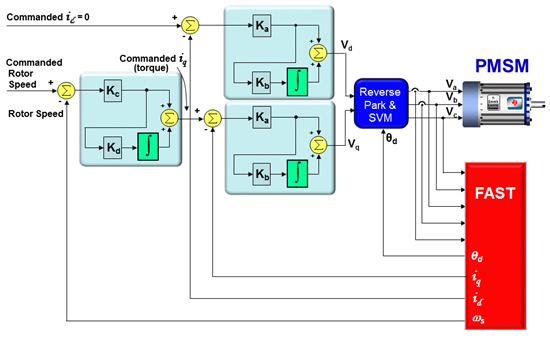
\includegraphics[width=0.8\linewidth]{09/01}
    \caption{Typical FOC Speed Control of a PMSM}
    \label{fig:09_01}
\end{figure}

The design of the velocity controller doesn’t change much in a field oriented system compared to other control algorithms.  But there are subtle differences which affect how you should design your current controllers, which are listed below.

\begin{enumerate}
    \item The motor’s equivalent RL circuit seen by the controllers (which determines how you set the PI coefficients) will vary depending on the motor type.  For BLDC and Permanent Magnet Synchronous Motors (PMSMs), $R$ is simply the stator resistance, and $L$ is the stator inductance.  As we have seen up to now, the PI coefficients are the same for the d and q current regulators.  But with AC Induction Motors (ACIMs), this is not the case.  For the d-axis, the resistance is equal to the stator resistance, just like it is with a PMSM.  But inspection of the rotor flux-based model of an AC induction motor reveals that the q-axis current controller sees an equivalent resistance equal to the stator resistance PLUS the rotor resistance.  Another difference is the inductance value you should use for both axes.  It turns out that it is not the stator inductance value, but rather the “series” inductance (or sometimes called the “leakage” inductance) which is defined as follows:

    \begin{equation}\label{eq:9_1}
        L = L_s \left(1-\frac{L_m^2}{L_sL_r}\right) = L_s \cdot \sigma
    \end{equation}
    where
    \begin{itemize}
        \item  $L$ = the equivalent series inductance
        \item  $L_s$ = the stator inductance
        \item  $L_m$ = the magnetizing inductance
        \item  $L_r$ = the rotor inductance
        \item  $\sigma$ = the “leakage factor” of the induction motor
    \end{itemize}

    Finally, it turns out that an IPM motor should be handled differently than either a PMSM or an ACIM.  The resistance value used by both the d and q axis current controllers is the stator resistance (just like any other PMSM).  The value used for inductance is the stator inductance, also similar to PMSMs.  But the stator inductance is different between the d and q axes, where $L_q$ is usually larger than $L_d$ due to the lower flux reluctance along that axis.

    In many cases these subtleties between motors won’t cause a big difference in the performance of your system, especially since you only have one pole in your current controller transfer function, and you can afford to be somewhat conservative.  But in higher performance, higher bandwidth systems, these subtleties must be considered, or you could end up with a PI current controller that is incompatible with your motor, resulting in less than optimal control.  As a first step in helping you manage all these different conditions, I have designed a \href{https://web.archive.org/web/20180101224106/http://e2e.ti.com/cfs-file/__key/telligent-evolution-components-attachments/13-852-00-00-00-66-49-89/PI-Calculator.xlsx?forcedownload=true}{spreadsheet} which can help you calculate the PI coefficients as a function of motor type for a field-oriented system.  The white cells represent fields that you must populate with data, and the grey cells will be calculated automatically based on the data you enter.  Go ahead and try it!  Just be mindful to use the correct SI units listed in each column, or you will not get the results you want.

    \item  It turns out that the control of the d-axis and q-axis currents are not independent from one another.  Within the motor, there is a natural cross coupling between the d-axis and q-axis which can be seen in the differential equations below for a PMSM:

    \begin{align}
        i_d \left(R+DL_s\right) &= V_d + \omega L_s i_q  \label{eq:9_2}\\
        i_q \left(R+DL_s\right) &= V_q - \omega \left(L_s i_d + K_e\right) \label{eq:9_3}
    \end{align}
    where
    \begin{itemize}
        \item $R$ is the stator resistance
        \item $L_s$ is the stator inductance
        \item $D$ is the differential operator
        \item $\omega$ is the electrical frequency
        \item $K_e$ = the Back EMF constant
    \end{itemize}

    From \ref{eq:9_2} we see that $V_d$ is not the only voltage term vying for control of the d-axis current.   There is also a speed dependent term which contains $i_q$ in it.  From \ref{eq:9_3}, $V_q$ is also competing with a voltage term containing $i_d$.  For both regulators, this cross-coupling effect manifests itself as an unwanted disturbance which is most prominent during transient conditions at high speeds.  To correct for this situation, feed-forward decoupling can be applied to each axis which exactly cancels these cross-coupled voltage terms.  The result is the regulator topology shown in Figure \ref{fig:09_02}.
\begin{figure}[H]
    \centering
    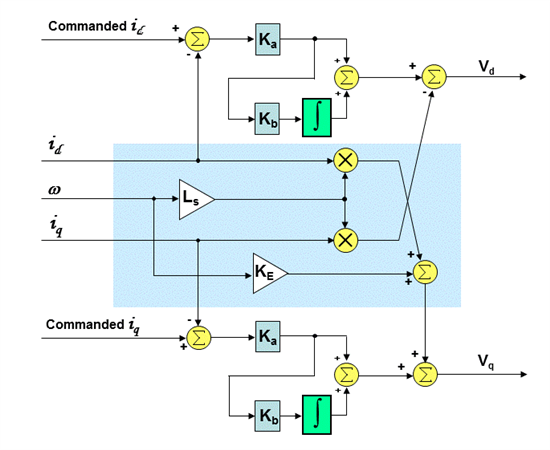
\includegraphics[width=0.8\linewidth]{09/02}
    \caption{Decoupled PI Controllers for a PMSM}
    \label{fig:09_02}
\end{figure}

    For AC Induction Motors, the correction becomes a little bit more sophisticated.  The differential equations defining AC induction motor operation are shown below:

    \begin{align}
        i_d \left(R_s+DL_s\sigma\right) &= V_d + \omega L_s \sigma i_q -\frac{L_m}{L_r}D\lambda_{rd} \label{eq:9_4}\\
        i_q \left(R_s+DL_s\sigma\right) &= V_q - \omega L_s \sigma i_d - \omega \frac{L_m}{L_r}\lambda_{rd} \label{eq:9_5}
    \end{align}
    where
    \begin{itemize}
        \item $R_s$ = the stator resistance
        \item $L_s$ = the stator inductance
        \item $\sigma$ = the leakage factor defined in \ref{eq:9_1}
        \item $D$ is the differential operator
        \item $\omega$ =  the electrical frequency
        \item $L_m$ = the magnetizing inductance
        \item $L_r$ = the rotor inductance
        \item $\lambda_{rd}$ = the d-axis rotor flux
    \end{itemize}

    Similar to the situation with a PMSM machine, we see that there are other voltages besides $V_d$ and $V_q$ vying for control of $i_d$ and $i_q$ respectively.  As a result, compensation voltages must be added to $V_d$ and $V_q$ to nullify these other voltage terms.  The compensation block used to provide correction voltages to the outputs of the $i_d$ and $i_q$ regulators is shown in Figure \ref{fig:09_03}.

    \begin{figure}[H]
        \centering
        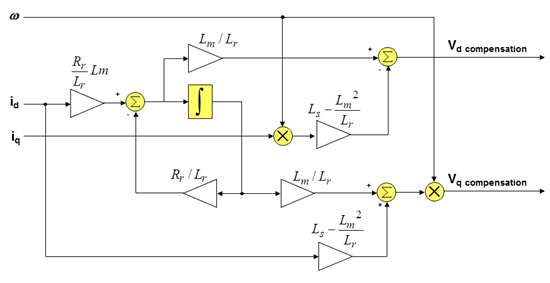
\includegraphics[width=0.8\linewidth]{09/03}
        \caption{Compensation Block used for Axis Decoupling with ACIMs.}
        \label{fig:09_03}
    \end{figure}

    As an example of the effectiveness of this technique, consider the simulation results of figure \ref{fig:09_04} which show the $i_d$ and $i_q$ waveforms for a 3 HP AC induction machine.  Without axis decoupling you can see how transient changes in $i_q$ current spill over into the d-axis.  This deviation from the commanded d-axis current will also cause an undesirable perturbation in the motor’s flux.  In the bottom graph we can see that the q-axis regulator is also ineffective at regulating $i_q$ during sudden changes in velocity.  But when the decoupling scheme of figure \ref{fig:09_03} is enabled, $i_d$ and $i_q$ currents track their respective commanded values much more precisely.


    \begin{figure}[H]
        \centering
        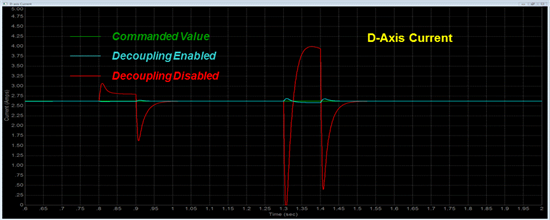
\includegraphics[width=0.8\linewidth]{09/04}
        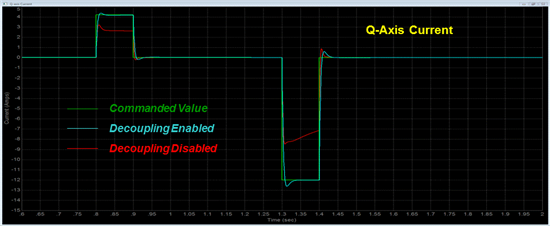
\includegraphics[width=0.8\linewidth]{09/05}
        \caption{Id and Iq Waveforms with and without Axis Decoupling.}
        \label{fig:09_04}
    \end{figure}

    A final thought about coupling compensation.  If you examine figures \ref{fig:09_02} and \ref{fig:09_03} you can see that what we are really doing is applying feed-forward signals to both the d and q regulator outputs.  The good news is that since this doesn’t add any poles to your closed-loop system, it is inherently stable.  But a word of caution\dots the feed-forward paths can inject very high frequencies from one axis into the other.  In some cases, this can excite your system with unwanted high frequency harmonics which can cause unwanted and unexpected behavior. This is especially true if you are operating the motor in field-weakened mode at high speeds.  Under these conditions you typically want to “handle with care”, or you can temporarily lose control of the motor.
\end{enumerate}

In my next and final blog entry on this topic, I would like to offer some concluding remarks regarding developing and debugging this PI tuning technique in a digital control system, as well as investigate the case where viscous damping is present.  In the meantime\dots


Keep Those Motors Spinning,\\

\includegraphics[width=0.2\linewidth]{01/04_dave}
\vfill
\textit{Apr 30 2013 17:32 PM}
\newpage
\textbf{UPDATE  July 19th, 2013}:  There have been several questions related to how I calculate the back-EMF constant ($K_e$) in my equations.  Several individuals have tried to use my \href{https://web.archive.org/web/20180101224106/http://e2e.ti.com/cfs-file/__key/telligent-evolution-components-attachments/13-852-00-00-00-66-49-89/PI-Calculator.xlsx?forcedownload=true}{spreadsheet} with their motor designs, only to obtain incorrect results which can be traced back to how $K_e$ is represented.

It turns out that the units for $K_e$ in my \href{https://web.archive.org/web/20180101224106/http://e2e.ti.com/cfs-file/__key/telligent-evolution-components-attachments/13-852-00-00-00-66-49-89/PI-Calculator.xlsx?forcedownload=true}{spreadsheet} are “volts (peak, line-to-neutral) per electrical radian per second”.  By representing $K_e$ in SI units like this, its numerical value is equivalent to the motor flux (in Webers).  Unfortunately, very few (if any) motor manufacturers represent back-EMF this way.  This means that you must convert your datasheet value for $K_e$ into the above units in order for the spreadsheet to yield correct results.  For example, Teknic Inc (as well as many other motor manufacturers) represents the back-EMF for their PMSM machines in volts (peak) per 1k RPM.  In just about every case, it is implied that this voltage is line-to-line since you usually can’t directly measure the line-to-neutral voltage.  To convert from these units to the SI units used in my spreadsheet, you must use the following multiplication factor:
\begin{equation*}
    \frac{\sqrt 3}{50 \pi P}
\end{equation*}
where P is the number of rotor poles.

The following multiplication factors can be used to convert the back-EMF units most frequently found on motor data sheets into the SI units in my spreadsheet:

\begin{tabular}{cc}
    \textbf{\underline{To convert from}} & \textbf{\underline{Multiply by}}\\
    Volts(peak, line-to-line) per electrical Hz  & $\frac{1}{2\pi\sqrt3}$ \\
    Volts(peak, line-to-line) per electrical radian/sec &  $\frac1{\sqrt 3}$\\
    Volts(peak, line-to-line) per mechanical radian/sec  & $\frac2{P\sqrt 3}$ \\
    Volts(peak, line-to-line) per kRPM & $\frac{\sqrt 3}{50\pi P}$ \\
    Volts(RMS, line-to-line) per electrical Hz & $\frac{1}{\pi \sqrt 6}$ \\
    Volts(RMS, line-to-line) per electrical radian/sec & $\sqrt{\frac{2}{3}}$ \\
    Volts(RMS, line-to-line) per mechanical radian/sec & $\frac{2}{P}\sqrt{\frac{2}{3}}$ \\
    Volts(RMS, line-to-line) per kRPM & $\frac{\sqrt 6}{50 \pi P}$ \\
\end{tabular}